% Asset ID: AS1EquationsInequalitiesTikZ-001
% Source: CCEA AS1-AF-LO004, AS1-AF-LO007, AS1-AF-LO014, AS1-AF-LO015;
%         P1 Chapter 3 PDF simultaneous equations using graphs section;
%         Chapter 3 transcript explanation of graph intersections and the discriminant.
% Related lesson section: Core Theory: Graph Intersections and the Discriminant.
% Purpose: Clean exam-style graph showing a line and a quadratic intersecting twice.
% Notes: This supports the example 2x + y = 3 and y = x^2 - 3x + 1.
%        Intersections are (-1,5) and (2,-1).
\documentclass[tikz,border=8pt]{standalone}
\usepackage{amsmath}
\usepackage{tikz}
\usetikzlibrary{arrows.meta}
\begin{document}
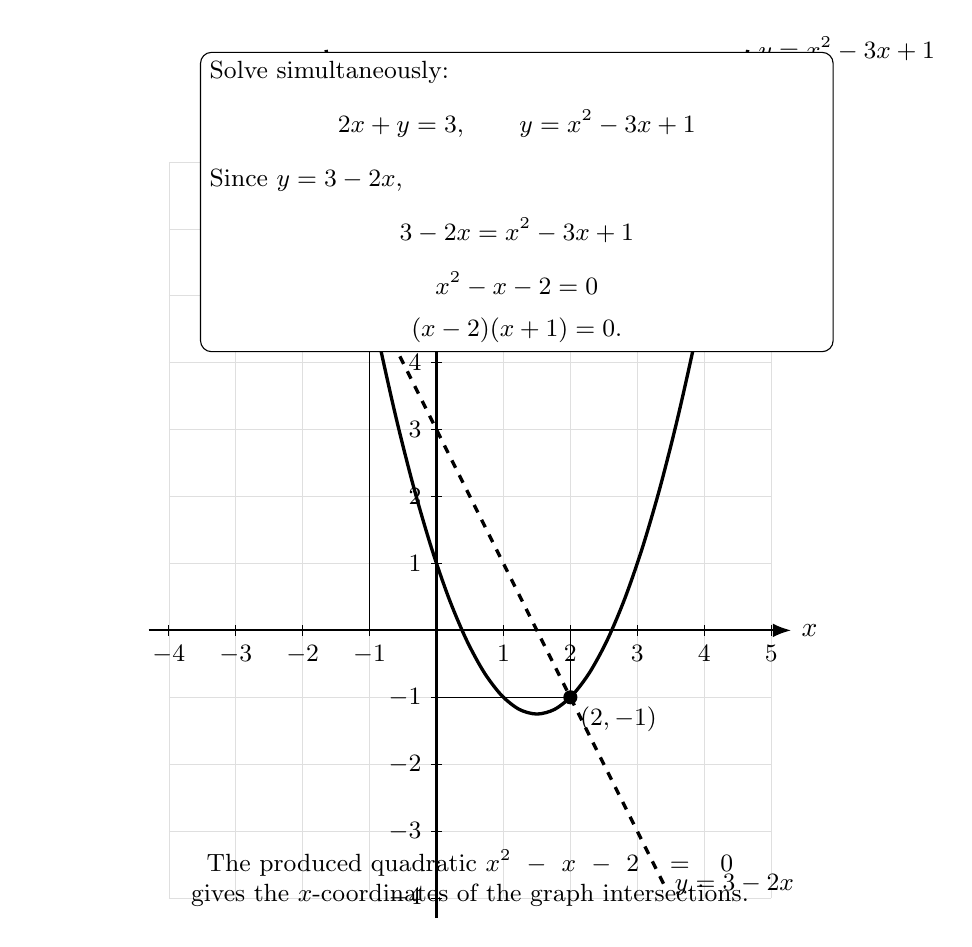
\begin{tikzpicture}[scale=0.85, >=Latex]
  \draw[step=1, very thin, gray!25] (-4,-4) grid (5,7);
  \draw[->, thick] (-4.3,0) -- (5.3,0) node[right] {$x$};
  \draw[->, thick] (0,-4.3) -- (0,7.3) node[above] {$y$};
  \foreach \x in {-4,-3,-2,-1,1,2,3,4,5} \draw (\x,0.08) -- (\x,-0.08) node[below, font=\small] {$\x$};
  \foreach \y in {-4,-3,-2,-1,1,2,3,4,5,6,7} \draw (0.08,\y) -- (-0.08,\y) node[left, font=\small] {$\y$};
  \draw[domain=-1.65:4.65, smooth, variable=\x, very thick] plot ({\x},{\x*\x - 3*\x + 1}) node[right, font=\small] {$y=x^2-3x+1$};
  \draw[domain=-2.1:3.4, smooth, variable=\x, very thick, dashed] plot ({\x},{3 - 2*\x}) node[right, font=\small] {$y=3-2x$};
  \fill (-1,5) circle (3pt); \fill (2,-1) circle (3pt);
  \draw[thin] (-1,0) -- (-1,5); \draw[thin] (0,5) -- (-1,5);
  \draw[thin] (2,0) -- (2,-1); \draw[thin] (0,-1) -- (2,-1);
  \node[above left, font=\small] at (-1,5) {$(-1,5)$};
  \node[below right, font=\small] at (2,-1) {$(2,-1)$};
  \node[draw, rounded corners, align=left, fill=white, text width=7.8cm, font=\small] at (1.2,6.4) {Solve simultaneously:
    \[2x+y=3,\qquad y=x^2-3x+1\]
    Since $y=3-2x$,
    \[3-2x=x^2-3x+1\]
    \[x^2-x-2=0\]
    \[(x-2)(x+1)=0.\]};
  \node[align=center, font=\small, text width=11cm] at (0.5,-3.7) {The produced quadratic $x^2-x-2=0$ gives the $x$-coordinates of the graph intersections.};
\end{tikzpicture}
\end{document}
